
\section{CPDOC information systems}\label{sec:cpdoc}

% CPDOC is a major center for teaching and research in the social
% sciences and contemporary history and is located in Rio de
% Janeiro. CPDOC is also a leading historical research institute in the
% country and it holds a major collection of personal archives, oral
% histories and audiovisual sources pertaining to Brazilian contemporary
% history.  CPDOC's private historical archival program hosts more than
% 1,8 million documents ranging from politics to economics, cultural
% history to social movements, and public policy to foreign
% relations. Over the years \mbox{CPDOC} has gathered a massive
% collection of oral histories. The historical archival program is
% mainly composed of three major information systems:

% \begin{itemize}
% \item Personal Archives: About 200 archival collections, comprising
%   approximately 1,8 million documents, including text, images and
%   videos.
% \item Oral History Program: A large set of testimonies (in audio and
%   video) consisting of more than 1.000 interviews, which corresponds
%   to roughly five thousand hours of recordings.
% \item Brazilian Historical Biographic Dictionary (DHBB): in the
%   current version, it consists of 7.553 entries, of which 6.584 are of
%   a biographical nature and 969 related to institutions, events and
%   concepts of interest for Brazilian history after 1930.
% \end{itemize}

% That is, the CPDOC data collection is storage in three distinct
% information systems developed originally for query and maintainance of
% three different databases. Each of these systems has independent
% management and adopts idiosyncratic criteria for the organization and
% indexing of your information. The data model vary according to the
% specific content of that they hold.

% Figure~\ref{fig:cpdoc-today} presents the CPDOC current
% architecture. The archives are maintained in three different
% information systems (the users interface of all of them are web-based)
% that share a common relational database. CPDOC's web portal provides a
% unify query interface for the archives metadata and low resolution of
% digital files. Each of the systems has independent management and
% adopts idiosyncratic criteria concerning the organization and indexing
% of the information, which vary depending on the specifications of the
% content they host: personal archives documents, oral history
% interviews and the Brazilian Historical -- Biographic Dictionary
% entries. CPDOC's web portal provides a unifying query interface. In
% the following subsections we briefly describe the systems.

Figure~\ref{fig:cpdoc-today} presents the current CPDOC database
architecture. The archives are maintained in three different
information systems that share a common relational database. 
Each of the systems has independent management and
adopts idiosyncratic criteria concerning the organization and indexing
of the information, which vary depending on the specifications of the
content they host: personal archives documents, oral history
interviews and the Brazilian Historical -- Biographic Dictionary
entries. CPDOC's web portal provides a query interface to archives data. In
the following subsections we briefly describe each of the systems.

\begin{figure}[thbp]
  \centering
  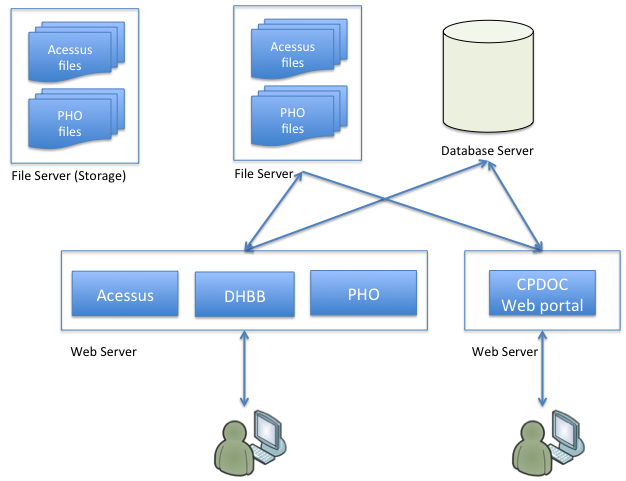
\includegraphics[width=.7\textwidth]{cur-architecture.png}
  \caption{CPDOC's current architecture}\label{fig:cpdoc-today}
\end{figure}

\subsection{Personal Archives (Acessus)}

This system is composed by personal
files from people who influenced the political and social scenario of
our country. These historical documents, in textual or audiovisual form, 
%are precious sources of knowledge that help us to know deeper our history. They may be 
in form of handwritten and printed texts, diaries, letters,
photographs, speeches or memos, represent much more than private
memories: they are the registry of a whole collective memory.

Currently, more than 200 personal archives from
presidents, ministers, military personal and other Brazil's important
public figures compose the CPDOC's collections. Together, they
comprise nearly 1.8 million documents or 5.2 millions pages. From
this, nearly 700 thousands pages are in digital format and the
expectance is to digitize all collections in the next few years. The
collection entries metadata are stored in an information system called
Acessus. It can be accessed through the institution's intranet for
data maintenance or by internet for simple data query.
% that provides and web interface in the FGV's intranet for data query,
% insert, delete and update. The web interface also provides simple
% reports generation interfaces.
Currently, allowed queries are essentially syntactic, i.e.,
% The reports and queries are
restricted to keywords searches linked to specific database fields
defined in an \emph{ad hoc} manner. For those documents that are
already digitized, two digital file versions were generated: one in
high resolution aiming long-term preservation and another in low
resolution for web delivery. High resolution files are stored in a storage system
with disk redundancy and restricted access, while low resolution files
are stored in a file
server~\footnote{\url{https://en.wikipedia.org/wiki/File_server}.}
(Figure~\ref{fig:cpdoc-today}).
% stores the low resolution versions of the digital files
% The files of the already digitalized documents are stored in two
% separated file
% servers~\footnote{\url{https://en.wikipedia.org/wiki/File_server}.}. One
% of them is a storage system with disk redundancy that stores the high
% resolution version of the files for long-term preservation. These
% files are available to a limit number of people with authorized
% access. The second file server stores low resolution versions of the
% digitial files that were used by the web systems and CPDOC's portal
% (Figure~\ref{fig:cpdoc-today}).

\subsection{Oral History Interviews (PHO)}

The CPDOC collection of Oral History hosts currently more than 6.000
hours of recording, corresponding to nearly 2.000 interviews.  More
than 90\% of it, video or audio, are in digital format. For the time being,
two kinds of queries are available in the database: query by subject and
query by interviewed. Each interview record holds a brief technical
information and a summary with descriptions of the interview
themes in the order they appear in the record. Only 10\% of the
interviews are transcribed, and to access the audio/video content the
user is requested to come personally to CPDOC. 

Currently, CPDOC is
analyzing better ways of making this data available online,
considering different aspects such as the best format, use policies,
access control and copyrights.

As in the case of Acessus, the database actually stores only the
metadata about the interviews, while digitized recorded audios and
videos are stored as digital files in the file servers.


\subsection{Brazilian Historical-Biographic Dictionary (DHBB)}

The Brazilian Historical-Biographic Dictionary (DHBB) is certainly one
of the main research sources for contemporary Brazilian politicians
and themes. It contains more than 7.500 entries of biographic and
thematic nature, i.e., people, institutions, organizations and events
records carefully selected using criteria that measure the relevance
of those to the political history for the given period. The entries
are written evenly, avoiding ideological or personal
judgments. CPDOC researchers carefully revise all entries added to
ensure the accuracy of the information and a common style criteria.

%Since it was launched, the DHBB has been an important source of
%information for researches, supporting the drafting of numerous theses
%and dissertations. For instance, Michael Conniff, Director of Global
%Studies Program and Professor of History at San Jose State University
%(California, EUA), after conducting an interesting prosopographical
%study over a selection of biographies extracted from DHBB, could draw
%a profile of the politicians who occupied important positions in the
%government after 1930 \cite{conniff}. Every biographic entry follow a
%common structure of writing that brings all those information beside
%conjunctures of Brazilian history.

The DHBB's database stores few metadata concerning each entry,
and the query is limited to keywords within the title or text.

% \subsection{CPDOC portal and public access interface}

% The three systems presented above share a common relational
% database. The implementation was conceived so as to facilitate the
% construction of a single query interface over all CPDOC archives in
% the CPDOC's web portal. In CPDOC's web portal users are required to
% login in order to access data, and the query interface available in
% there is the only means for reach that.

%%% Local Variables: 
%%% mode: latex
%%% TeX-master: "article"
%%% End: 
